\documentclass[11pt,a4paper]{scrreprt}
\usepackage[utf8]{inputenc}
\usepackage[T1]{fontenc}
\usepackage{amsmath}
\usepackage{amsfonts}
\usepackage{amssymb}
\usepackage{graphicx}
\usepackage[width=42.00cm, height=59.40cm, left=2.00cm, right=2.00cm, top=2.00cm, bottom=2.00cm]{geometry}
\usepackage{babel}
\usepackage{blindtext}
\setlength{\parindent}{0pt} % Einrücken vom Text unterdrücken
\usepackage{wrapfig}% textumflossene Grafik
\usepackage{xcolor} % Farbe
\usepackage{hyperref}
\usepackage{enumitem}
\usepackage{colortbl}
\usepackage{pdflscape}
\usepackage{xcolor}
\usepackage{subfigure}
\newtheorem{Code_kurz}{Code  }[chapter]
\usepackage{caption}
\usepackage{float}


\begin{document}
		\titlehead{
		\begin{flushright}
			\includegraphics*{img/HTW_Logo_rgb}
		\end{flushright}
	}
	
	\title{Seminar - deep learning}
	\subtitle{price prediction real estate data from web scraping}
	\author{
		\textbf{Stephan Baartz} \\*[1em]
		\textbf{Matrikel-Nummer 548908}
	}
	\date{}
	\publishers{\textbf{Surveyor: \begin{tabular}[t]{l}
				Dr. Alla Petukhina
	\end{tabular}}\\*[3em]
	Submitted February 28, 2023}
\maketitle

	\tableofcontents
	\listoffigures
	\listoftables
	\thispagestyle{empty}
	\cleardoublepage\pagenumbering{arabic}
	
	\chapter{Introduction}\label{chap:Einleitung}
	Web scraping is a method of automatically extracting data from websites. This is done with the help of programs or scripts that analyze the HTML code of a website and extract specific data. In this seminar paper, data from Immonet.de for 20 different cities was extracted automatically. Information such as the cold and warm rent, as well as other data such as the condition or the type of property are available. The chapter \ref{sec:Webscraping} briefly discusses the topic of web scraping and the problems that arise in the process. The analysis of the data and the search for outliers is discussed in the chapter \ref{sec:Datenanalyse}.  Two different benchmark models are developed: a linear regression and a decision tree using gradient boosting (xgboost).  The linear model is briefly discussed in \ref{subsec: lineare Regression}, xgboost in \ref{subsec: xg}. These models will serve as benchmarks to verify whether the third model - the main part of this seminar paper - the neural network provides a better prediction for the cold and warm rents.  The programming language of this seminar paper is R and the neural network is created using the package 'neuralnet'. The choice of parameters and the adaptation of the neural network are not always clear, so in this elaboration a performance test is performed in parallel and different parameters are compared. At the end a bootstrap aggregation and an analysis of the predicted intervals is done.


	\chapter{Webscraping} \label{sec:Webscraping}
Web scraping is a method of automatically extracting content from web pages. The page from which the data is extracted is \hyperref[https://www.immonet.de/immobiliensuche/sel.do?suchart=2&fromarea=1.0&torooms=9999.0&city=87372&marketingtype=2&pageoffset=1&radius=0&parentcat=1&listsize=26&sortby=0&objecttype=1&fromrooms=1.0&fromprice=1.0&page=1]{}{}{}{immonet.de}\footnote{ It is important to use the correct URL, because the URL contains the filter settings and the information that the first page is displayed (Page-1). For example, a For loop can be used to access different pages. \hyperref[https://www.immonet.de/immobiliensuche/sel.do?suchart=2&fromarea=1.0&torooms=9999.0&city=87372&marketingtype=2&pageoffset=1&radius=0&parentcat=1&listsize=26&sortby=0&objecttype=1&fromrooms=1.0&fromprice=1.0&page=2]{}{}{}{https://www.immonet.de/immobiliensuche/sel.do?suchart=2\&fromarea=1.0\&torooms=9999.0\&city=87372\& marketingtype=2\&pageoffset=1\&radius=0\&parentcat=1\&listsize=26\&sortby=0\&objecttype=1\&fromrooms=1.0\& fromprice=1.0\&page=1}}. Some filter settings were used to exclude unfavorable data from the outset:

\begin{description}
	\item[Ort] Used as a variable during readout. For example Berlin\footnote{In the URL the code city=87372 is used for this purpose}.
	\item[Was] Exclusively apartments - no houses or land 
	\item[Preis] from  1 EUR -  some rental prices are only communicated 'on request'. With the filter these properties will be ignored.
	\item[FLäche] from  $1 \ m^2$ -  For the calculation of a price per square meter, the area is essential
	\item[Zimmer] 1 - 999 - In order to prevent possible problems with the readout from the outset
\end{description} 

The website immonet.de delivers 444 hits for Berlin at the time of writing this seminar paper. There is an ID for each property. With this unique ID, the concrete property can be called up in turn. This unique ID ultimately provides the URL of the apartment and can be determined as follows:

\begin{verbatim}
	page<-read_html("https://www.immonet.de/immobiliensuche/sel.do?suchart=2&
	fromarea=1.0&torooms=9999.0&city=87372&marketingtype=2&
	pageoffset=1&radius=0&parentcat=1&listsize=26&sortby=0&
	objecttype=1&fromrooms=1.0&fromprice=1.0&page=1")
	page %>%
	html_elements(".flex-grow-1.overflow-hidden.box-25 a")%>%
	html_attr("href")
\end{verbatim}

This results in 26 ID's for the first page.
\begin{verbatim}
	ids
	1  /angebot/47032733
	2  /angebot/49369370
	3  /angebot/49357545
	.
	.
	.
	24 /angebot/49187554
	25 /angebot/49178201
	26 /angebot/48180027
\end{verbatim}

The combination of the URL immonet.de and the first ID provides the URL immonet.de/angebot/47032733 to a specific property. The URL is used to get to the properties of the real estate. This procedure was carried out for 20 cities. This resulted in a total of 6520 data records on 23.12.2022. The verification of the correctness of the data revealed some problems that will be addressed in the rest of the paper.


\section{Problems of the data set}

After the data set was completely extracted, the data was checked for plausibility. In the process, some errors were noticed on the website. Before the check, a definition for the warm rent and the cold rent had to be created.

The warm rent refers to the rent including all ancillary costs and the heating costs. Also included are any costs for garage parking spaces. The cold rent, on the other hand, viewed from the perspective of an investor, represents the return on the property. Since ancillary costs and heating costs must be borne by the tenant, the cold rent is defined as rent without any other costs.

Inconsistencies were noticed when reviewing the data.

\subsection{Warm rent = cold rent}
Somewhat unusual is the fact that for some properties the warm rent corresponded to the cold rent. Upon closer inspection, it turned out that these were either furnished apartments or student or senior housing with assisted living. Flat rents are nothing unusual in this context. Basically, this is not an error of the data set, but a limitation of the readout process, since this information is only available as text and an additional analysis of the texts would have been necessary to extract this information. 

\begin{figure}[H]
	\centering
	
\includegraphics[width=0.7\linewidth]{img/49069527}
	\caption{Error: warm rent = cold rent}
	\label{fig:49069527}
\end{figure}

\subsection{Cold rent > Warm rent}

The cold rent was greater than the warm rent. Initially, the assumption was that the data had not been read out correctly. However, after closer examination, it could be determined that the operators of Immonet.de do not check the data for plausibility before publishing the advertisement. As can be seen in the figure \ref{fig: error kalt > warm} for example, the ID's 47122153 and 48642772 provide a larger cold rent than warm rent. This is obviously wrong, but a closer look shows that warm and cold rent were swapped here. In total, there were 5 records that were incorrect in this area. 4 records were corrected and one was removed. 

\begin{figure}[H]
	\begin{center}
		\begin{minipage}{0.4\textwidth}
			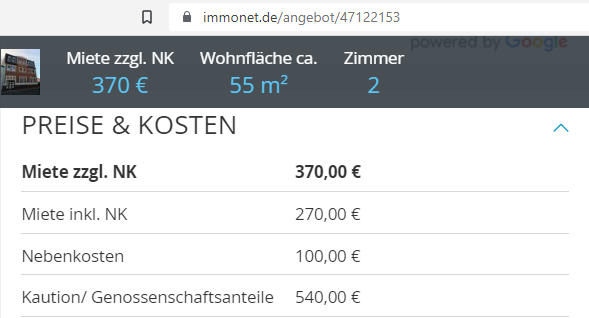
\includegraphics[width=0.7\linewidth]{img/47122153}
		\end{minipage}
		\begin{minipage}{0.4\textwidth}
			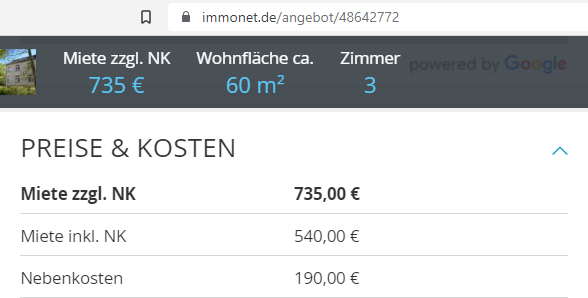
\includegraphics[width=0.7\linewidth]{img/48642772}
		\end{minipage}
	\end{center}
	\caption{Error: Cold rent > Warm rent }
	\label{fig: error kalt > warm}
\end{figure}

\subsection{Heating costs included in warm rent}
The page offers two fields to determine whether the heating costs are included in the warm rent or in the service charges or not. Quite obviously, there are problems of confusion here. The figure \ref{Error: Heizkosten in Warmmiete} shows that the difference between warm rent and cold rent is the same as the indicated heating costs. It can be assumed that in these cases the heating costs are included in the service charges instead of in the warm rent as indicated.
\begin{figure}[H]
	\begin{center}
		\begin{minipage}{0.4\textwidth}
			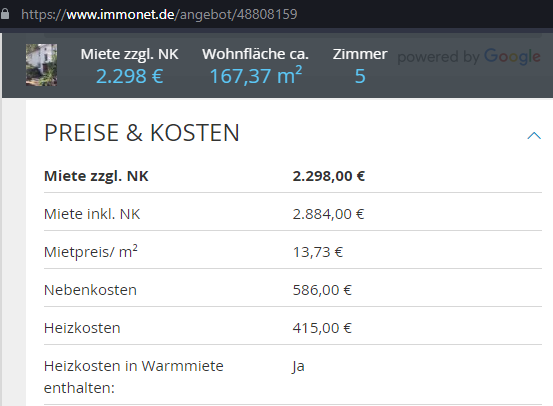
\includegraphics[width=0.7\linewidth]{img/48808159}
		\end{minipage}
		\begin{minipage}{0.4\textwidth}
			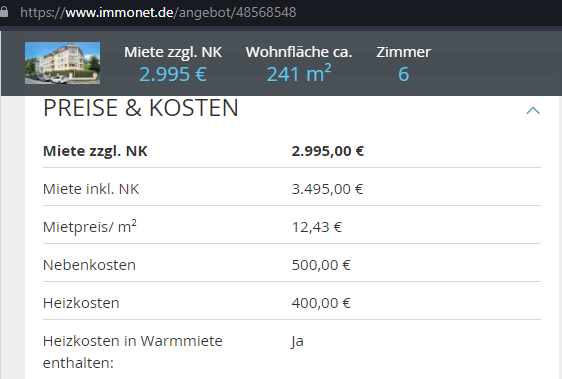
\includegraphics[width=0.7\linewidth]{img/48568548  }
		\end{minipage}
	\end{center}
	\caption{Error: Heating costs = ancillary costs?  }	
	\label{Error: Heizkosten in Warmmiete}
\end{figure}

In addition, there are problems with the query whether the heating costs are included in the service charges. The figure \ref{fig: Heikosten in NK} shows that the sum of cold rent and service charges does not correspond to the warm rent. It is likely that the figure indicates that the heating costs are included in the warm rent.

\begin{figure}[H]
	\centering
	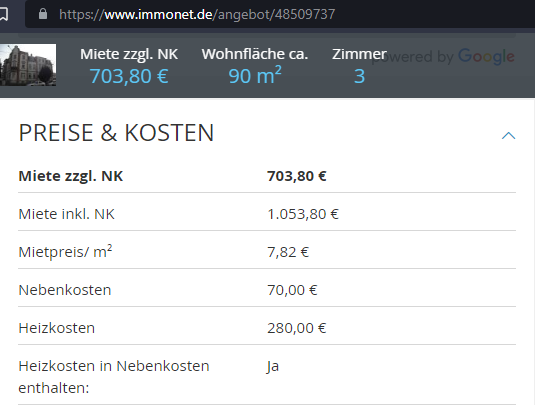
\includegraphics[width=0.7\linewidth]{img/48509737}
	\caption{Error:  Heating costs in ancillary costs}
	\label{fig: Heikosten in NK}
\end{figure}


\subsection{Garage}

An additional problem is the indication of the garage. There are cases when garage parking spaces belong to a property and the price for this parking space is specified. In some cases the price of the garage parking space is included in the cold rent, in other cases it is not. There are also cases where the price for the garage parking space is included in the warm rent, in other cases it is not. These data have been corrected, if it was possible, to ensure the correctness of the data. 



\subsection{Interim summary}

The initial analysis of the data highlighted a flawed data set. Some differences between cold and warm rent could not be clearly determined. Often, the erroneous difference was only a few euros. These errors were accepted because they may not have been significant enough to affect the analysis. Some data were still wrong despite all assumptions, which is illustrated by the figure \ref{Error: allgemeine Fehler}.  However, this type of error can be corrected by the subsequent outlier analysis. It should be noted that the poor quality of the data did not result from the readout, but that the operators of Immonet.de did not have the data checked by a program before publication. Only a few additional queries would be required to significantly improve the data quality. The fact that the data quality is poor could cause problems in the modeling. The following is an analysis of the data set first.

\begin{figure}[H]
	\begin{center}
		\begin{minipage}{0.4\textwidth}
			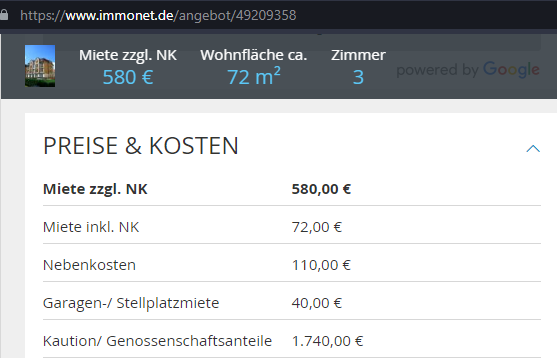
\includegraphics[width=0.7\linewidth]{img/49209358}
		\end{minipage}
		\begin{minipage}{0.4\textwidth}
			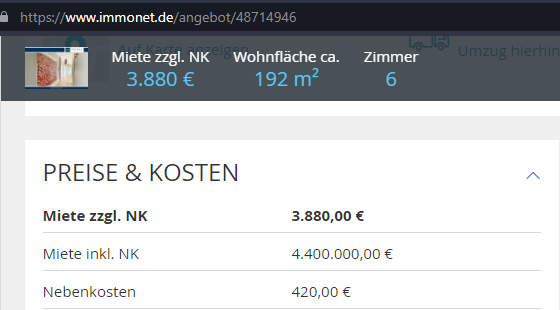
\includegraphics[width=0.7\linewidth]{img/48714946  }
		\end{minipage}
	\end{center}
	\caption{Error: Heating costs = ancillary costs? }
	\label{Error: allgemeine Fehler}
\end{figure}
		\chapter{Data Analysis}\label{sec:Datenanalyse}
In this seminar paper, an analysis of apartment prices in 20 German cities is conducted. The data set was obtained by webscraping from the website Immonet.de and contains information such as size, price, number of rooms and location of the apartments. In the first step of the data analysis, the dataset is described to gain an understanding of the data. In the second step, potential outliers are identified and examined using statistical methods and graphical representations to identify unusual or implausible data. 


\section{Description of the data set}

To get an optimal overview of the data set the form of a table was chosen. The table \ref{tbl: vor der Analyse} shows the data set before the analysis. For this purpose, the following column headings were chosen. 
\begin{description}
	\item[Variable] The name of the  variables 		
	\item[Str] The structure of the variables. Thereby stands:
	\begin{description}
		\item[fac] for factors or categorical variables
		\item[chr] For Character - 'Text' variables
		\item[num] Numerical data
		\item[date] Date format
		
	\end{description}
	\item[Number/levels] For numeric values, it is the number of records. For categorical data, it is the number of categories
	\item[Median] The median of the numerical data
	\item[Range] For categorical variables, the different categories are indicated with the number of available data for the corresponding category. The prerequisite is that a categorical variable has less than 10 values. For numerical data, the smallest and largest value is output
	\item[NA] NA stands for not available. These data were not specified in the advertisements.
	\item[Note] Personal note
	
\end{description}

\begin{landscape}
	\begin{tabular}{|l||c|c|c|l|l|l|} \hline
		Variable         & str  & Number/levels & Median	    	& Range                          & NA & Anmerkung\\ \hline \hline
		Warmmiete      	 & num  & 6520                & 1021      	& 200 - 19.850             & - & \\  \hline
		Kaltmiete      	 & num  & 6520                & 793      	& 72 - 17.000              & - & \\   \hline
		ID               & chr  & 6520                &			    	& -                              & - & The unique ID \\ \hline
		Zimmer           & num  & 6520                & 2  	    	& 1 - 10                         &-  & Number of rooms\\ \hline
		Fläche           & num  & 6520                &	72.5$m^2$    	& 7 - 706                    & - & The area of a property\\ \hline
		Ort      		 & fac	& 727                  &				    & Adlershof ... Zehlendorf       & - & The district is not used \\ \hline
		Zustand    		 & fac	& 11                  &				    & Altbau... Vollsaniert          & - & The condition of a property  \\ \hline
		Art              & fac  & 9                   &    				& Apartment: 531                 & - & The type of property\\ 
		&      &                     &	    			& Dachgeschosswohnung: 621       & &\\
		&      &                     &    				& Erdgeschosswohnung: 617        & &\\
		&      &                     &    				& Etagenwohnung: 2822          & &\\
		&      &                     &	    			& Loft-Studio-Atelier: 25        & &\\
		&      &                     &	    			& Maisonette: 184                & &\\
		&      &                     &	    			& Penthouse: 90                 & &\\
		&      &                     &	    			& Souterrainwohnung: 30          & &\\
		&      &                     &	    			& Wohnung: 1600                   & &\\ \hline
		Fotos 		    & num  & 6520                &	10	    		& 0 - 42                         & - & The number of photos provided \\ \hline
		Baujahr         & Date & 168                 & 1960   			& 0022 - 2024                    & 1179 &  Year of construction of the property\\ \hline
		Denkmalschutz   & bool & 2                   &	    			& True: 180                      & & If not specified: FALSE \\ 
		&      &                     &    				& False: 6340                    & & \\ \hline
		Energieklasse   & fac  & 9                   &    				& Klasse A+ - Klasse H           & 3595 & A+ best energy class, H worst   \\ \hline
		Energieverbrauch& num  &                     &	95  kWh/(m²*a)& 1 - 62.755                    & 2597  & Outlier! \\ \hline
		Energieverbrauchsausweis & fac  & 3                   &	                 & Energiebedarfsausweis: 1990   &  &If "nicht nötig"    \\ 
		&      &                     &	                 & Energieverbrauchsausweis: 2080  &  1952 &  -> no energy consumption specified \\ 
		&      &                     &	                 & nicht nötig:498               &     &\\ \hline
		Heizungsart & fac  & 3                   &	                 & Etagenheizung: 429            & 2570 &     \\ 
		&      &                     &	                 & Zentralheizung: 3511          &    &  \\ 
		&      &                     &	                 & Ofenheizung: 10          &     & \\ \hline
		Befeuerungsart  & fac  & 41                  &	                 & Erdwärme,Solar... Gas         & 1254 & Many combinations of energy types \\ \hline
		Dokumente       & num  & 6520                &	  0             & 0-9           		         & - & The number of documents provided \\ \hline
	\end{tabular}
	%\caption{Datensatz vor der Analyse}
	\label{tbl: vor der Analyse}
\end{landscape}
\section{Outlier analysis}\label{sec:Ausreißeranalyse}

The outlier analysis is used to detect possible deviations or errors in the data set. Identifying outliers can ensure that the results of the analysis are valid and based on a stable database. It allows to improve the data quality by removing or correcting these outliers. Thus, the goal of outlier analysis is to check the data for plausibility and thereby increase the reliability and validity of the results. 

A correlation plot is a statistical tool used to show the relationships between different numerical variables in a data set. A correlation plot can be used to quickly see if there are correlations between variables and how strong those correlations are. To get started with a correlation plot, all numeric data is plotted in a matrix. This matrix is converted into a correlation plot that visualizes the relationships between all variables \cite{Korrelations Matrizen}. Using colors and markers, one can quickly see which variables are strongly correlated and which variables may be outliers. The figure \ref{fig: korrelationVorher}  shows the correlation plot before the outlier analysis. 

\begin{figure}[h!]
	\centering
	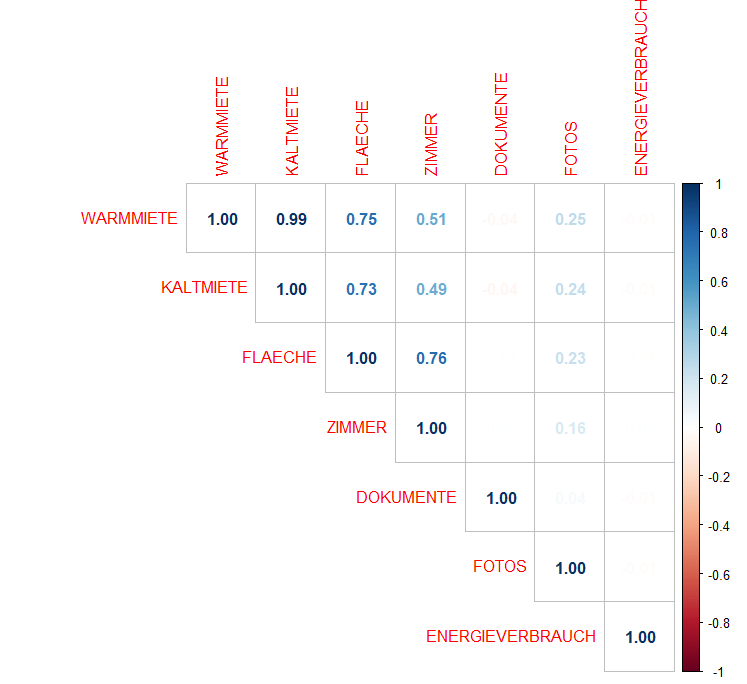
\includegraphics[width=0.7\linewidth]{img/korrelationVorher}
	\caption{Correlation plot before outlier analysis}
	\label{fig: korrelationVorher}
\end{figure}

It can be seen that the correlation between the warm rent and the cold rent is 99\% and that the area and the number of rooms show a very strong correlation with the rent price. This is plausible, since, as a rule, a larger apartment should also be more expensive. In addition, the correlation of almost 0 between the warm rent and energy consumption suggests that there could be erroneous data or outliers here. At this point, there could be a negative correlation, so that the rent becomes cheaper when the energy consumption is very high. Since the number of pages of this seminar paper is limited, not every feature will be discussed separately in the following. However, the problems that have arisen will be discussed using three examples. 


\subsection{Target variable warm and cold rent}

Based on the quantiles in table \ref{tbl: Quantile Warm- und Kaltmiete} and the fact that the range of rents is very large, it was decided to use a logarithmic representation in \ref{fig: log warm und kaltmiete}.

\begin{table}[H]
	\begin{verbatim}
		> summary(tbl$warmmiete)
		Min. 1st Qu.  Median    Mean 3rd Qu.    Max. 
		200     705    1021    1328    1614   19850 
		
		> summary(tbl$kaltmiete)
		Min. 1st Qu.  Median    Mean 3rd Qu.    Max. 
		72.0   519.8   793.2  1062.1  1303.7 17000.0 
	\end{verbatim}
	\caption{Quantiles of cold and warm rent}
	\label{tbl: Quantile Warm- und Kaltmiete}
\end{table}
In this chart, the so-called 'heavy tails' are clearly visible. There are some very low and very high rents that distort the plot. These data points were initially identified as outliers, but not yet removed so as not to influence the other characteristics in advance.

\begin{figure}[H]
	\subfigure[Cold rent]{\includegraphics[width=.45\linewidth]{"img/log kaltmiete"}}
	\subfigure[Warm rent]{\includegraphics[width=.45\linewidth]{"img/log warmmiete"}}
	\caption{Comparison of the cheapest and most expensive property }
	\label{fig: log warm und kaltmiete}
\end{figure}

\subsection{Area}

A part from the very strong correlation between the warm and cold rent, the highest correlation was recorded for the area. In the following, due to the high correlation between the warm and cold rent, only the warm rent is considered. Strange area values can also be seen for the area. The smallest property has an area of 7 $m^2$, the largest property is 706 $m^2$. These two properties were also marked as outliers. Figure  \ref{fig: fläche log warm} shows the root area and log warm rent including the outliers. It has been found that the adjusted $R^2$ has deteriorated in the logarithmic plot compared to the normal plot. It also showed that the $R^2$ of the root representation also deteriorated compared to the normal representation, but only minimally. Therefore, the root representation was initially chosen for the area.

\begin{figure}[H]
	\centering
	\includegraphics[width=0.7\linewidth]{img/fläche log warm}
	\caption{log warm rent and root area}
	\label{fig: fläche log warm}
\end{figure}


\subsection{Energy consumption, year of construction and energy class}

There are several problems for the features energy consumption, year of construction and energy class. First, there is some missing and incorrect data in the data and second, this analysis should ultimately be used to calculate a potential rental price for tenants or landlords. This results in the challenge that for a tenant, for example, the actual year of construction is not of interest, but a time period in which the property was built. Incorrect data also shows construction years from 0022, so data prior to 1700 was classified as missing data. To solve the problem of converting to a categorical variable, the KMEANS algorithm\footnote{\cite{KMEANS} S.8)} was used to calculate the optimal clusters. The missing data were then categorized as an additional category of 'Not specified'. This approach was applied to all three variables.
The figure \ref{fig: Baujahr Warmmiete boxplots} shows that the median warm rent increases as the age of the property increases.
\begin{figure}[H]
	\centering
	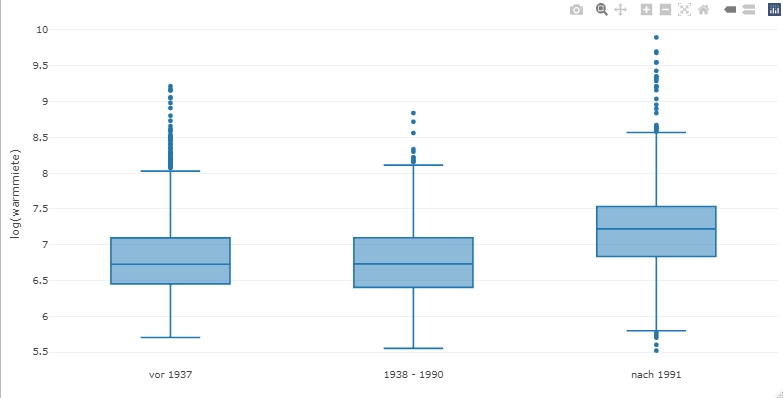
\includegraphics[width=0.7\linewidth]{img/Baujahr Warmmiete boxplots}
	\caption{Year of manufacture cluster boxplots}
	\label{fig: Baujahr Warmmiete boxplots}
\end{figure}
There are several reasons why the median warm rent might increase as the property ages. One possible reason could be that older buildings are usually less energy efficient and therefore incur higher energy costs, which can affect the rent price. Another reason could be that older buildings tend to be less modernized and therefore less attractive to tenants, which can also affect the rent price. It could also be that older buildings are simply in better locations or more popular neighborhoods and therefore have higher rents\footnote{At this point, further research could be conducted}.

\section{Interim summary}
Some interesting findings were obtained through the outlier analysis. On the one hand, it was found that the correlations between the numerical data were hardly improved by the different transformations (e.g. log or root representation). On the other hand, additional erroneous data came to light that had previously gone undetected. This erroneous data was classified as missing data and some features were transformed into categorical data. The Mahalonobis distance\footnote{For the mathematical basis be referred to \cite{Mahalonobis} and \cite{Mahalonobis2} Af page 325 and 326} was also calculated for the numerical data of warm rent, cold rent, area and number of rooms. This yielded 53 outliers, which are shown in Figure \ref{fig: Maha Ausreißer}.However, it turned out that the correlation between the variables nevertheless did not improve. 

\begin{figure}[H]
	\subfigure[Outlier log room and log price]{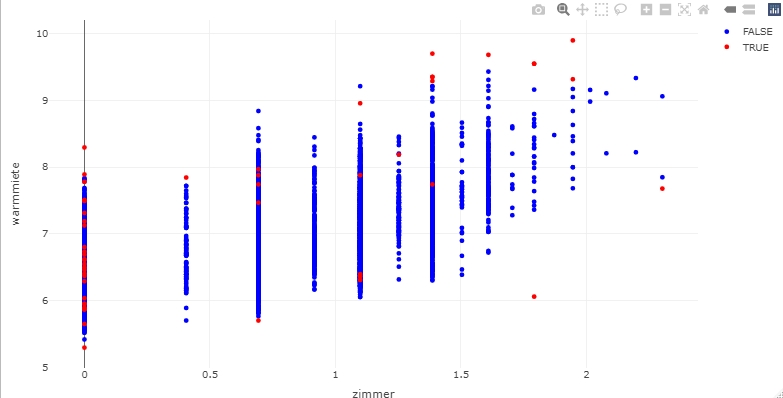
\includegraphics[width=0.3\linewidth]{img/maha zimmer Preis}}
	\subfigure[Outlier log area and log price]{\includegraphics[width=0.3\linewidth]{img/maha fläche Preis}}
	\subfigure[Outlier log area and log room]{\includegraphics[width=0.3\linewidth]{img/maha zimmer fläche}}
	\caption{Mahalanobis distance outlier}
	\label{fig: Maha Ausreißer}
\end{figure}
The correlations are shown in Figure \ref{fig: Korrelation nach der analyse}  dt can be seen that the correlation with energy consumption has improved signifikant. However, this is negligible because the data was transformed into a categorical variable. Also, the correlations for what are probably the most important features (area and room) have worsened rather than improved. For this reason, no outliers were ultimately removed. Nevertheless, the analysis was useful to correct erroneous data and stabilize the data set. With the entire 6520 data, development of various models will begin in Section 4. The correlation are shown in \ref{chapter: Modell}. 
\begin{figure}[h!]
	\centering
	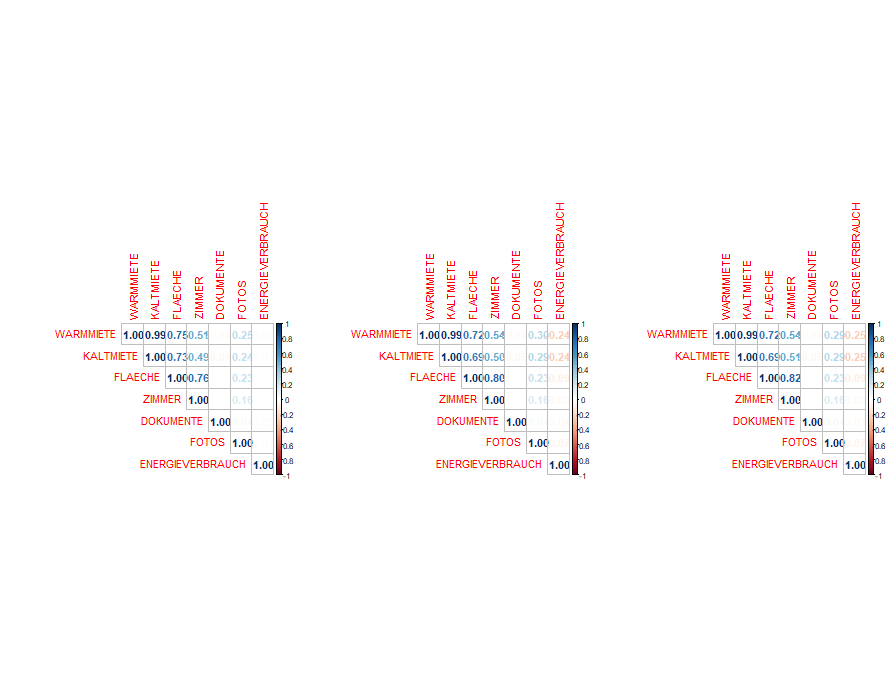
\includegraphics[width=0.9\linewidth]{img/Korrelation nach der analyse}
	\caption{Correlation plot after outlier analysis}
	\footnotesize\sffamily (Left before analysis, center log/root plot, right without outliers and log/root plot.) 
	\label{fig: Korrelation nach der analyse}
\end{figure}

		\chapter{Modell} \label{chapter: Modell}
	In this paper, the prediction of rental price intervals is investigated using statistical and machine learning methods. In particular, the focus is briefly on the application of linear regression and decision trees. This focus is necessary to obtain a comparative model for a neural network developed later. For this purpose, the data set is divided into training and test data in a ratio of 80:20.  An accuracy dataset is also created documenting the error functions ME (Mean Error), RMSE (Root Mean Squared Error), MAE (Mean Absolute Error), MPE (Mean
	Percentage Error) and MAPE (Mean Absolute Percentage Error). The focus is on the RMSE. In addition, the name of the model and the runtime (in minutes) are added to the data set. The column 'Warm rent' documents whether the Accuracy values refer to warm or cold rent. The column 'Train\_test' documents whether the Accuracy values refer to the training or test data. In addition, 'Seed' is listed to allow the data to be reproduced. The empty data set that is filled with the following models is of the following shape:

	\begin{table}[H]
	\begin{verbatim}
		ME RMSE MAE MPE MAPE                     Name  Zeit Warmmiete train_test seed
		-----------------------------------------------------------------------------
	\end{verbatim}
	\caption{Accuracy table: empty data set}
	\label{tbl: lm-Modell}
\end{table}

	\section{Linear regression} \label{subsec: lineare Regression}
	Linear regression is a simple and widely used statistical model used to explain a dependent variable in terms of one or more independent variables. It assumes that there is a linear relationship between the variables \cite{LM}. In this paper, an attempt is made to predict rental prices based on various characteristics of the apartments, such as size, location and condition of the apartment. To do this, we first develop a linear regression model for warm rent that represents rent prices as a function of characteristics.
	The anova analysis for the first linear model found that the features documents, firing type, and flat rent had no significant effect on the model. After removing these data and running a regression again, the result was the table\ref{tbl: lm-Modell}. This first table suggests that linear regression in this form does not provide good predictions for the test data. The model fits the training data much better than the test data. However, it is not possible to make a final assessment of the model until a comparative model has been constructed.
	
	\begin{table}[H]
		\begin{verbatim}
    ME RMSE MAE MPE MAPE                     Name  Zeit Warmmiete train_test seed
    -----------------------------------------------------------------------------
    20  628 231  -2   16                       Lm   0.0      TRUE      train   NA
   -19 1247 243  -3   16                       Lm   0.0      TRUE       test   NA
    21  619 231  -2   16 Lm   - PM - BevArt - Dok   0.0      TRUE      train   NA
   -19 1234 243  -3   16 Lm   - PM - BevArt - Dok   0.0      TRUE       test   NA	
		\end{verbatim}
	\caption{Accuracy table: lm-Modell}
	\label{tbl: lm-Modell}
	\end{table}
	
	\section{XGBoost} \label{subsec: xg}
	XGBoost (Extreme Gradient Boosting) XGBoost belongs to the class of gradient boosting algorithms and combines several weak models into a strong decision tree. In this work, many small trees with a maximum branch depth of 3 are generated. A single tree is extremely weak. The combination of several trees leads to an extremely efficient and strong model.  (vgl. \cite{Data Science Solutions with Python} p.66 and \cite{XG}	).
	The following code shows how to perform cross-validation using XGBoost. First, the optimal number of trees is evaluated and then the final model is created \footnote{Again the note: The number of pages of this term paper is limited. The focus will be on the neural network, so it is not possible to go into details here.}.	
	
	\begin{verbatim}
		param<-list(
		objective = "reg:linear",
		booster = "gbtree",
		eta=0.05, # should prevent overfitting default 0.3
		gamma=0, # 0 - oo - the larger the more conservative  
		max_depth=3, #default=6  - larger trees -> overfitting + speicer problems
		min_child_weight=1, #default=1
		subsample=1
		)
		xgbcv <- xgb.cv( 
		   params = param, 
		   data = xgtrain, 
		   nrounds = 2000, 
		   nfold = 5, # Equal sized samples
		   showsd = T, 
		   stratified = T, 
		   print_every_n = 40,
		   early_stopping_rounds = 10, # if no further improvement -> abort
		   maximize = F, 
		   base_score = .5,
		   prediction = T)
		xgb_mod <- xgb.train(data = xgtrain, params=param, nrounds = xgbcv$best_iteration,base_score =.5)
	\end{verbatim}

\begin{table}[H]
	\begin{verbatim}
   ME RMSE MAE MPE MAPE                     Name  Zeit Warmmiete train_test seed
   -----------------------------------------------------------------------------
   20  628 231  -2   16                       Lm   0.0      TRUE      train   NA
  -19 1247 243  -3   16                       Lm   0.0      TRUE       test   NA
   21  619 231  -2   16 Lm   - PM - BevArt - Dok   0.0      TRUE      train   NA
  -19 1234 243  -3   16 Lm   - PM - BevArt - Dok   0.0      TRUE       test   NA
  -----------------------------------------------------------------------------
   18  204 118  -1    9                   xg 648   0.6      TRUE      train  123
   14  547 189  -2   13                   xg 648   0.6      TRUE       test  123	
	\end{verbatim}
	\caption{Accuracy table: xg-Modell}
	\label{tbl: xg-Modell}
\end{table}

The Accuracy data were added to the table  \ref{tbl: xg-Modell}. Based on the second model, it is already clear how poor the linear regression model actually is. Moreover, based on the test data, the RMSE of 547 EUR is a good value to compete with the neural network. The model is discussed in more detail in section \ref{sec:NN}.

\section{Neural networks}\label{sec:NN}

Now, the rental prices are studied using neural networks. In particular, the R package 'neuralnet' is used to develop a neural network capable of predicting rental prices based on various characteristics of the apartments. The Rprop+ algorithm is used to train and optimize the neural network. Rprop+ is a further development of the Rprop algorithm used for neural network training. It is a so-called 'on-line' optimizer, meaning that it performs weight adjustments during training, rather than before training as in batch optimizers \cite{Riedmill NN 1993}. The Rprop+ algorithm is based on the fact that the learning rate adjusts independently for each weight. Unlike other optimizers such as gradient descent, which adjusts the learning rate for all weights simultaneously, Rprop adjusts the learning rate for each weight individually. It also uses an 'adaptive' learning rate, which means that the learning rate for each weight is adjusted based on the last change in the weight \cite{Ruder NN rprop+}.
Neural networks have emerged in recent years as powerful tools for predicting target variables. They have the ability to learn complex relationships between inputs and outputs, and are able to model nonlinear relationships between features and rent. For the activation function of the neural network used in this work, the logistic function (also called sigmoid function) \ref{Formel: logistic}  was chosen\footnote{Other functions can also be used. The sigmoid function has the advantage that it is defined on the interval 0-1}.

\begin{align}\label{Formel: logistic}
	\sigma(x) = \frac{1}{1 + e^{-x}}
\end{align} 
Here $x$ is the input of the function and $\sigma(x)$ is the output, which is between 0 and 1. This function has the advantage that it restricts the output of the network to a value between 0 and 1, which is advantageous for predictions of probabilities. The rents are previously scaled to an interval between 0 and 1 using the min-max transformation.

\begin{align}
	X_{norm} = \frac{X - X_{min}}{X_{max} - X_{min}}
\end{align}
Where $X$ is the original value ( e.g. rental price), $X_{min}$ is the smallest value of the training data of a variable, $X_{max}$ is the largest value of the training data of a variable and $X_{norm}$ is the normalized value of the variable. It is important to note that the training and test data were each scaled using the max-min values of the training data. This is necessary so that a single data set can be predicted at the end.

The error function used in this work was the Root Mean Squared Error (RMSE). This error function calculates the root mean squared error between the actual and predicted values. 

A neural network with one layer and one neuron was first created. Surprisingly, already the first neural network gave better results than all models before\footnote{based on the RMSE}, so the run was repeated with a different seed, as shown in Table \ref{tbl: nn-Modell I}. 

\begin{table}[H]
	\begin{verbatim}
   ME RMSE MAE MPE MAPE                     Name  Zeit Warmmiete train_test seed
   -----------------------------------------------------------------------------
   20  628 231  -2   16                       Lm   0.0      TRUE      train   NA
  -19 1247 243  -3   16                       Lm   0.0      TRUE       test   NA
   21  619 231  -2   16 Lm   - PM - BevArt - Dok   0.0      TRUE      train   NA
  -19 1234 243  -3   16 Lm   - PM - BevArt - Dok   0.0      TRUE       test   NA
  -----------------------------------------------------------------------------
   18  204 118  -1    9                   xg 648   0.6      TRUE      train  123
   14  547 189  -2   13                   xg 648   0.6      TRUE       test  123
   -----------------------------------------------------------------------------
   37  481 227  -2   15                  nn c(1)   2.2      TRUE      train    1
   23  423 214  -3   15                  nn c(1)   2.2      TRUE       test    1
   37  483 226  -2   15                  nn c(1)   0.5      TRUE      train    2
   22  397 211  -3   15                  nn c(1)   0.5      TRUE       test    2	
	\end{verbatim}
	\caption{Accuracy table: nn-Modell I}
	\label{tbl: nn-Modell I}
\end{table}

However, it should be noted that one layer and one neuron might not be enough for a more complex problem and it is recommended to add more layers and neurons to improve the performance of the model \cite{Deep Learning Goodfellow}. Therefore, another experiment was performed by creating a layer with two neurons. The results are shown in Table \ref{tbl: nn-Modell II}.

\begin{table}[H]
	\begin{verbatim}
   ME RMSE MAE MPE MAPE                     Name  Zeit Warmmiete train_test seed
   -----------------------------------------------------------------------------
   20  628 231  -2   16                       Lm   0.0      TRUE      train   NA
  -19 1247 243  -3   16                       Lm   0.0      TRUE       test   NA
   21  619 231  -2   16 Lm   - PM - BevArt - Dok   0.0      TRUE      train   NA
  -19 1234 243  -3   16 Lm   - PM - BevArt - Dok   0.0      TRUE       test   NA
  -----------------------------------------------------------------------------
   18  204 118  -1    9                   xg 648   0.6      TRUE      train  123
   14  547 189  -2   13                   xg 648   0.6      TRUE       test  123
   -----------------------------------------------------------------------------
   37  481 227  -2   15                  nn c(1)   2.2      TRUE      train    1
   23  423 214  -3   15                  nn c(1)   2.2      TRUE       test    1
   37  483 226  -2   15                  nn c(1)   0.5      TRUE      train    2
   22  397 211  -3   15                  nn c(1)   0.5      TRUE       test    2
   -----------------------------------------------------------------------------
   35  475 224  -2   15                  nn c(2)   0.4      TRUE      train    1
   20  395 210  -3   15                  nn c(2)   0.4      TRUE       test    1
   32  450 213  -2   15                  nn c(2)   1.0      TRUE      train    2
   15  417 209  -3   15                  nn c(2)   1.0      TRUE       test    2 	
	\end{verbatim}
	\caption{Accuracy table: nn-Modell II}
	\label{tbl: nn-Modell II}
\end{table}

Interestingly, the runtimes do not increase significantly in these first examples. Furthermore, it cannot be clearly determined whether a neural network with two neurons is better than a neural network with one neuron. The results depend on the randomly chosen weights and the other hyperparameters\footnote{The hyperparameters were always identical in order to compare the models. Generally speaking, the result naturally depends on the hyperparameters}. Therefore, in the further course of the experiment, different more complex neural networks are investigated in order to evaluate the performance. For this purpose, the following networks were chosen arbitrarily:

\begin{itemize}
	\item c(4,2) - 2 layers with 4 and 2 neurons 
	\item c(5,3) - 2 layers with  4 and 3 neurons
	\item c(3,2,1) - 3 layers with  3, 2 and one neurons
	\item c(6,3,2) - 3 layers with  6,3 and two neurons
\end{itemize}

\section{Forecast} \label{sec: prediction}

	The table \ref{tbl: nn-Modell III} is interesting from several points of view. On the one hand, it is clear that the running times increase. The neural network with 3 layers and six, three and one neuron ran for 12.6 minutes. The seed data also indicates that it took three runs for the neural network to converge. Thus, the 12 minutes is deceiving, as the first two runs ran longer than 12 minutes without obtaining a valid model. A neural network may not converge for several reasons, such as the initial values of the weights, the number of neurons, the learning rate, and the choice of error function. In this case, the network could not converge because the learning rate was set too high or the number of maximum passes (100,000) was set too low. Thus, the weights could not reach an optimal minimum. It should also be noted that the results (RMSE) did not clearly improve based on the test data. The models clearly depend on the initial values. To deal with this problem, bootstrap aggregation was performed.


\begin{table}[H]	
	\begin{verbatim}
   ME RMSE MAE MPE MAPE                     Name  Zeit Warmmiete train_test seed
   -----------------------------------------------------------------------------
   20  628 231  -2   16                       Lm   0.0      TRUE      train   NA
  -19 1247 243  -3   16                       Lm   0.0      TRUE       test   NA
   21  619 231  -2   16 Lm   - PM - BevArt - Dok   0.0      TRUE      train   NA
  -19 1234 243  -3   16 Lm   - PM - BevArt - Dok   0.0      TRUE       test   NA
  -----------------------------------------------------------------------------
   18  204 118  -1    9                   xg 648   0.6      TRUE      train  123
   14  547 189  -2   13                   xg 648   0.6      TRUE       test  123
  -----------------------------------------------------------------------------
   37  481 227  -2   15                  nn c(1)   2.2      TRUE      train    1
   23  423 214  -3   15                  nn c(1)   2.2      TRUE       test    1
   37  483 226  -2   15                  nn c(1)   0.5      TRUE      train    2
   22  397 211  -3   15                  nn c(1)   0.5      TRUE       test    2
  -----------------------------------------------------------------------------
   35  475 224  -2   15                  nn c(2)   0.4      TRUE      train    1
   20  395 210  -3   15                  nn c(2)   0.4      TRUE       test    1
   32  450 213  -2   15                  nn c(2)   1.0      TRUE      train    2
   15  417 209  -3   15                  nn c(2)   1.0      TRUE       test    2 
  -----------------------------------------------------------------------------
   25  379 189  -2   13                nn c(4,2)   7.7      TRUE      train    1
    1  374 201  -3   15                nn c(4,2)   7.7      TRUE       test    1
   24  397 193  -2   13                nn c(4,2)   6.9      TRUE      train    3
   -1  586 210  -3   15                nn c(4,2)   6.9      TRUE       test    3	
  -----------------------------------------------------------------------------
   22  344 176  -1   13                nn c(5,3)   6.0      TRUE      train    2
   16  485 214  -3   15                nn c(5,3)   6.0      TRUE       test    2
  -----------------------------------------------------------------------------
   28  404 195  -2   14              nn c(3,2,1)   3.0      TRUE      train    3
   11  415 201  -3   15              nn c(3,2,1)   3.0      TRUE       test    3
  -----------------------------------------------------------------------------
   21  346 173  -1   12              nn c(6,3,2)  18.1      TRUE      train    1
    6  399 201  -3   15              nn c(6,3,2)  18.1      TRUE       test    1
   24  380 175  -1   12              nn c(6,3,1)  12.6      TRUE      train    3
   -1  461 217  -3   16              nn c(6,3,1)  12.6      TRUE       test    3
  -----------------------------------------------------------------------------
	\end{verbatim}
	\caption{Accuracy table: nn-Modell III}
	\label{tbl: nn-Modell III}
\end{table}
	
	
	\subsection{Bootstrap Aggregation} \label{subsec: boot}
	Bootstrap aggregation (also called bagging) is a technique used to reduce the uncertainty of estimates by creating random subsets from the original dataset \cite{Bootstrap}. This method creates new datasets by selecting random data with layback from the existing training dataset. The result is a collection of models trained on different data. In this case, bootstrap aggregation was used to reduce the uncertainty of the estimates and improve the results. The training dataset consisted of 5215 records. Thus, 5215 data sets were pulled from the training dataset in each run with layback and six different models were created.


	 \begin{itemize}
	 	\item c(1) one layer and one neuron
	 	\item c(2) one layer and two neurons
	 	\item c(3) one layer and three neurons
	 	\item c(4,1) two layers with 4 and one neuron
	 	\item c(4,2) two layers with 4 and two neurons
	 	\item c(4,3) two layers with 4 and three neurons
	 \end{itemize}
	 
	 For the first three models, 50 runs were selected. However, due to run time, only 20 runs were selected for the last three models. A data matrix with 210 columns and 5215 rows was created. The first 50 columns refer to the first model, the next 50 columns refer to the second model, and so on. When the mean of the first 50 columns is calculated, the result is a more stable prediction for a model with one layer and one neuron. The results for the test data are shown in Table \ref{tbl: bagging}.

	          

\begin{table}[H]
 	\begin{verbatim}
   ME  RMSE   MAE  MPE MAPE   Name Mean.Zeit Warmmiete train_test Durchlaeufe Konvergiert
   --------------------------------------------------------------------------------------
 21.7 406.0 213.0 -2.6 15.5   c(1)       3.4      TRUE       Test          50          50
 18.8 388.0 207.0 -2.7 15.1   c(2)       4.1      TRUE       Test          50          33
 1.9  342.0 190.0 -3.0 14.3   c(3)       8.0      TRUE       Test          50          33
 8.6  379.0 189.0 -3.1 14.0 c(4,1)       9.7      TRUE       Test          20          14
-1.9  363.0 192.0 -3.6 14.4 c(4,2)      14.1      TRUE       Test          20          11
 1.9  340.0 188.0 -3.1 14.2 c(4,3)      12.1      TRUE       Test          20          14
   --------------------------------------------------------------------------------------
 20.8 350.4 190.7 -3.3 17.9   c(1)       3.4     FALSE       Test          50          50
 21.6 345.2 187.2 -3.2 17.6   c(2)       4.1     FALSE       Test          50          33
 2.0  334.3 173.2 -3.7 16.5   c(3)       8.0     FALSE       Test          50          33
 7.8  320.0 168.2 -3.8 16.1 c(4,1)       9.7     FALSE       Test          20          14
-1.3  315.5 170.4 -4.4 16.6 c(4,2)      14.1     FALSE       Test          20          11
 3.5  302.8 168.0 -3.7 16.4 c(4,3)      12.1     FALSE       Test          20          14
    --------------------------------------------------------------------------------------
 	\end{verbatim}
 \caption{Bootstrap Aggregation}
 \label{tbl: bagging}
\end{table}

	It can be seen that the average runtime of a model increases significantly when the number of neurons and layers is increased. Moreover, it can be seen that only the model with one layer and one neuron never had problems with convergence. It converged in 50 out of 50 trials. In percentage terms, more models converged for the more complex models c(4,1) and c(4,3) than for the models with two and three neurons and one layer, respectively. The c(4,2) model had the most difficulty, with only 55 \% converged models. It is also observed that the more complex models with two shifts give better results for cold rent, while this is not necessarily the case for warm rent. One advantage of bagging that has not been mentioned so far is that prediction intervals can now be created. The equation shows the calculation \ref{Formel: VI}.

\begin{align}\label{Formel: VI}
	VI=\vec{\overline{x}} \pm a \cdot \vec{s_x}
\end{align} 

	Where $\vec{s_x}$ is the vector of standard deviations of each data set and $\vec{\overline{x}}$ corresponds to the arithmetic mean of the forecasts. The value $a$ is not clearly defined in the literature and depends on what the prediction is intended to achieve. In this work, the value 1 and 2 were tested first and then it was decided to use 1.5, so that on the one hand the intervals do not become too large and there is enough data in the interval. It was also decided to use only the last 60 models with two layers, on the basis of which the following prediction intervals were calculated.

\subsection{Prediction intervals}

	Based on the formula \ref{Formel: VI} results in some intervals that are relatively small and others that are very large. Relatively precise forecasts could be made for some data, but not for others. Figure \ref{fig: HIST VI} shows an example forecast interval where the actual price of a test data set is not in the forecast interval. In the further course, these are referred to as hits and no hits, respectively.


\begin{figure}[h!]
	\centering
	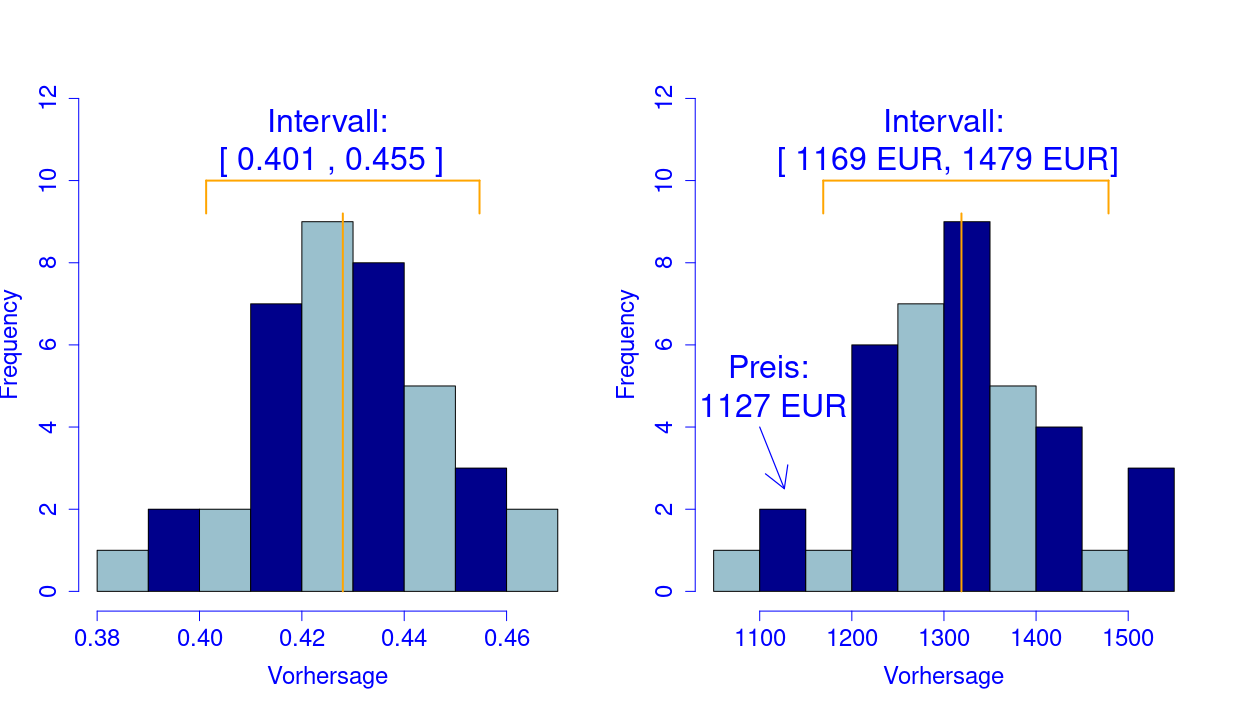
\includegraphics[width=.9\linewidth]{img/hist KI}
	\caption{Prediction interval. Left before the back transformation. Right after the back transformation}
	\label{fig: HIST VI}
\end{figure}

		For the entire test data, this modeling yields the five largest forecast intervals (warm rent) in table\ref{tbl: top 5 absolut}. Surprisingly, only one warm rent was predicted correctly. 

\begin{table}[H]
	\begin{verbatim}
  Tatsächlicher Preis Unteres Intervall Oberes Intervall Treffer Differenz
1               19850             13000            17000   FALSE      4000
2               12450              9300            11000   FALSE      1700
3               11000              7600             8700   FALSE      1100
4                2300              3900             4800   FALSE       900
5                2700              2600             3400    TRUE       800
	\end{verbatim}
\caption{The five absolute biggest differences}
\label{tbl: top 5 absolut}
\end{table}

		For the five smallest absolute forecast intervals, the modeling also yielded only one hit out of five, as shown in Table\ref{tbl: top 5 absolut unten}.

\begin{table}[H]
	\begin{verbatim}
  Tatsächlicher Preis Unteres Intervall Oberes Intervall Treffer Differenz
1              470.00               470              490    TRUE        20
2              550.00               560              580   FALSE        20
3              558.28               510              530   FALSE        20
4              621.00               630              650   FALSE        20
5              629.00               570              590   FALSE        20
	\end{verbatim}
	\caption{The five absolute biggest differences}
	\label{tbl: top 5 absolut unten}
\end{table}

	The five largest and smallest differences in percentage terms are shown in table  \ref{tbl: top 5 relativ} and \ref{tbl: top 5 relativ unten}. The picture looks a little better for the largest percentage intervals. 

\begin{table}[H]
	\begin{verbatim}
  Tatsächlicher Preis Unteres Intervall Oberes Intervall Treffer Prozent
1                1300              1000             1600    TRUE      60
2                 628               690             1100   FALSE      59
3                1150              1000             1500    TRUE      50
4                1325              1000             1500    TRUE      50
5                 700               820             1200   FALSE      46
	\end{verbatim}
	\caption{The five largest differences in percentage terms}
	\label{tbl: top 5 relativ}
\end{table}


\begin{table}[H]
	\begin{verbatim}
  Tatsächlicher Preis Unteres Intervall Oberes Intervall Treffer Prozent
1             1000.75               980             1000   FALSE       2
2             1008.90               960              980   FALSE       2
3              981.15               950              970   FALSE       2
4              925.25               920              940    TRUE       2
5              837.00               900              920   FALSE       2
	\end{verbatim}
	\caption{The five smallest differences in percentage terms}
	\label{tbl: top 5 relativ unten}
\end{table}

 Overall, this analysis yields only 23 \% hits (294). In 40 \% of the data, the price was overestimated. In 37 \% of the data, the warm rent was underestimated. The residuals in Figure  \ref{fig: warmmiete qq}  clearly show that the model had difficulty with very large and very small rents.
 

\begin{figure}[H]
	\centering
	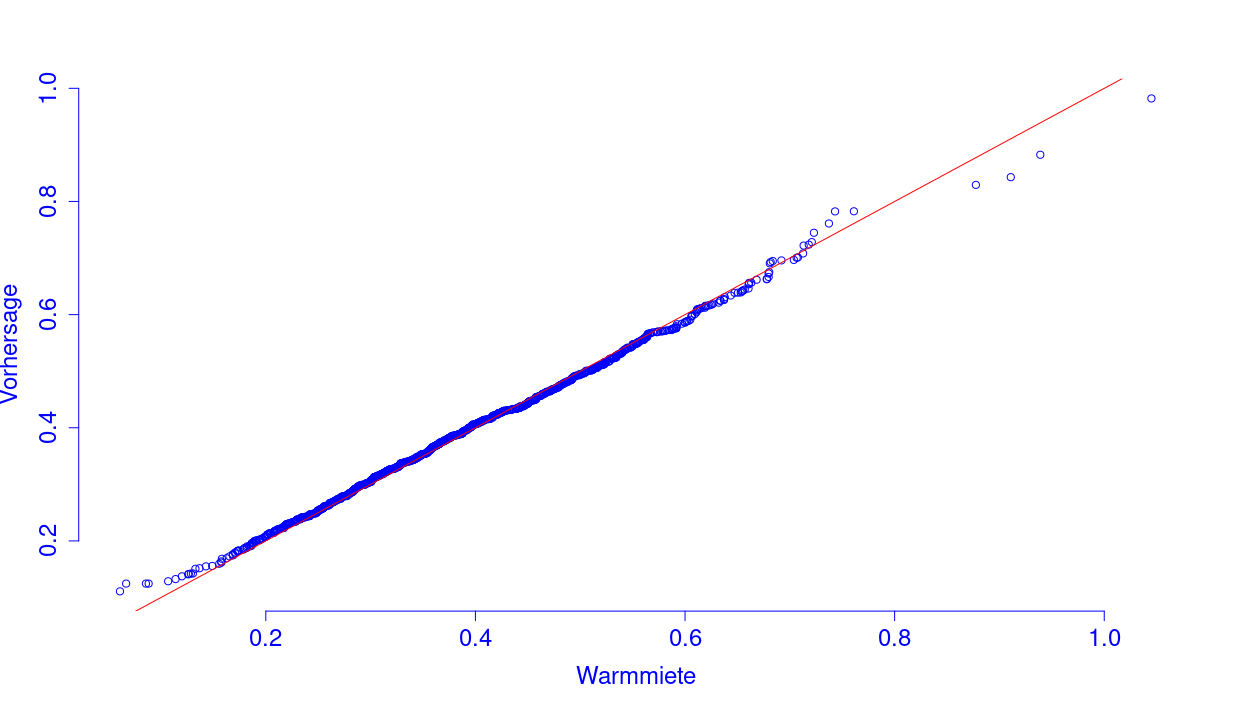
\includegraphics[width=.9\linewidth]{img/warmmiete qq}
	\caption{qqplot cold rent prediction vs. actual value}
	\label{fig: warmmiete qq}
\end{figure}


	\chapter{Summary} \label{sec: Fazit}
	The goal of this work was to make predictions for warm and cold rents based on real estate data that was read out via webscraping from immonet.de. The reading of the data worked well, but there were many erroneous data, which were discussed in chapter \ref{sec:Webscraping} . For example, there were cases where the cold rent was higher than the warm rent. These data were manually corrected once patterns were detected. The problems already indicated that prediction could be difficult. The outlier analysis also showed that there were other errors in the data, such as properties with year of construction 0022 or energy consumption greater than 60,000 $kWh/(m^2 \cdot a)$.	Some of these problems were solved by converting the affected data into categorical data, such as creating three and four classes, respectively, for year of construction, one of which was for missing data. Since the correlations before and after the analysis of the outliers did not improve, the outliers were not removed. Linear regression in section \ref{subsec: lineare Regression} and anova analysis were first performed, and the prediction for warm rent was very poor compared to the other models.  The decision tree in section \ref{subsec: xg} provided a better comparative model for the neural networks in section \ref{sec:NN}.Problems with convergence were noted and it was difficult to decide on a specific model. The subsequent bootstrap aggregation in section \ref{subsec: boot} brought some clarity. Based on these 210 models, the final decision was made to use the 60 more complex models, and based on this, a prediction interval was created for the test data. The analysis of the prediction intervals yielded sobering results with only 22 \% hits. The residual analysis indicated that the modeling had problems especially at the edges. In retrospect, the decision not to remove the outliers detected by the Mahalonobis distance may have been wrong. This might have resulted in better modeling of the residuals in the qq plot	 (figure \ref{fig: warmmiete qq}). For further investigations, even more complex models with more layers and more neurons may be possible. However, the documented runtime has to be considered. Already a model with two layers and four and two neurons ran on average 14 minutes. More complex models will increase the run times again. As an alternative to complexity, further investigation of the hyperparameters should be conducted. For example, an analysis of the learning rate could be performed. Other activation functions such as the tangent hyperbolic function could also be exploited. It would also be interesting to analyze how the model evolves when the number of iterations is changed. In the models used, a maximum of 100,000 iterations were performed. On the other hand, this will again affect the runtime.
	
	\begin{thebibliography}{9}
	\bibitem[BQ]{Bootstrap} Quinto, Butch. Next-Generation Machine Learning with Spark. New York, NY, Apress, [2020].
	ISBN 978-1-4842-5669-5
	
	\bibitem[IG]{Deep Learning Goodfellow} Ian Goodfellow and Yoshua Bengio and Aaron Courville.Deep Learning. MIT Press 2016. http://www.deeplearningbook.org
	
	\bibitem[KV]{Mahalonobis} Kurt Varmuza, Peter Filzmoser (2009). Introduction to Multivariate Statistical Analysis in Chemometrics. Taylor und Francis Inc. ISBN-13 978-1420059472
	
	\bibitem[MD]{KMEANS} Matthew F. Dixon, Igor Halperin, Paul Bilokon (2020). Machine Learning in Finance. From Theory to Practice. Springer Nature Switzerland AG. ISBN 978-3-030-41067-4 / e-ISBN 978-3-030-41068-1
	
	
	\bibitem[MF]{Korrelations Matrizen} Michael Friendly (2002). Corrgrams: Exploratory displays for correlation matrices. The American Statistician
	https://doi.org/10.1198/000313002533
	
	\bibitem[MK]{Applied Predictive Modeling} Max Kuhn. Springer. 1st ed. 2013, Corr. 2nd printing 2018 edition (17 May 2013).
	ISBN-13: 978-1461468486
	
	\bibitem[RM]{Riedmill NN 1993} Riedmiller, M. and Braun, H. (1993) A Direct Adaptive Method for Faster Backpropagation Learning: The RPROP Algorithm. Proceedings of the IEEE International Conference on Neural Networks, San Francisco, 28 March 1 April 1993, 586-591. {http://dx.doi.org/10.1109/ICNN.1993.298623} 
	
	\bibitem[SR]{Ruder NN rprop+}	Sebastian Ruder. An overview of gradient descent optimization algorithms. Insight Centre for Data Analytics, NUI Galway
	Aylien Ltd., Dublin. https://arxiv.org/abs/1609.04747
	
	\bibitem[TN]{Data Science Solutions with Python}  Nokeri, Tshepo Chris (2022). Data Science Solutions with Python. Berkeley, CA, Apress. ISBN 978-1-4842-7762-1.

	\bibitem[YD]{Mahalonobis2} Yadolah Dodge (2008) The Concise Encyclopedia of Statistics. Springer Verlag. 
	ISBN-13 978-0397518371
	
	\bibitem[CJ]{LM} Chambers, J. M., \& Hastie, T. J. (1992). Statistical Models in S. London: Chapman \& Hall. ISBN 9780412830402
	
	\bibitem[XG]{XG}	Group of community members. Official documentation XGBoost. https://xgboost.readthedocs.io/en/stable/
	
	
	
	


\end{thebibliography}
\end{document}